\documentclass[9pt,twocolumn,twoside]{opticajnl}
\journal{opticajournal}

\setboolean{shortarticle}{true}

\usepackage{lineno}
\usepackage{array,tabularx}

\title{Finite-size--corrected synchronization in a city-scale bus network:
crossover, not demonstrated criticality}

\author[1,*]{Po-Hsun Lai}
\affil[1]{Department of Physics, National Taiwan University, Taipei, Taiwan}
\affil[*]{b11202025@ntu.edu.tw}

\setboolean{displaycopyright}{false}
\doi{}

% Figures are the selected raw-data rebuild outputs retained in this repository.
\graphicspath{{../output/figures/}}
\newcommand{\rexc}{r_{\mathrm{exc}}}
\newcommand{\ppc}{\mathrm{PPC}}

\begin{abstract}
Bus bunching is often interpreted as phase synchronization whose onset occurs when passenger
demand exceeds a critical value.  We test this on 13.85 million GPS fixes and
6.79 million boarding records from 20 routes in Niter\'oi, Brazil.  The raw first Kuramoto--Daido
order parameter is not comparable across observations: under independent random phases its
baseline scales approximately as $0.886/\sqrt{N}$, while the median observed fleet contains only
six buses.  We validate same-$N$ Monte Carlo nulls against Kluyver's exact planar-random-walk
distribution and compare five normalizations, two phase definitions, and four null models.
Corrected order is positively associated with realized boardings per active bus, but only one of
three predeclared criticality signatures passes; a free-exponent scaling collapse is
optimizer-boundary and start-grid sensitive and is therefore not identified.  The appropriate
nearest-neighbour Newell--Potts model predicts instability for every positive load rather than a
positive threshold, although its measured load parameter does not predict which hourly cells
amplify.  Spatial position provides the dominant empirical reinterpretation: 51.37\% of active
bus-hours lie in the outer 10\% of a route, terminal order is nearly one, and interior corrected
order is $-0.189$.  The whole-route load coefficient is $0.0376$, whereas the interior coefficient
is $0.0011$ ($p=0.933$); direct control for terminal fraction attenuates the whole-route coefficient
by 44\%.  Shared-corridor coherence also falls toward zero after controlling shared-segment speed.
Thus an apparently Kuramoto-like field signal is not evidence of a city-scale critical transition:
it is substantially shaped by finite-fleet bias, boundary occupancy, inherited operational
irregularity, and common road-state shocks.
\end{abstract}

\begin{document}

\maketitle

\section{Introduction}

A delayed bus encounters passengers accumulated over a longer headway, dwells longer, and loses
more time; the following bus encounters fewer passengers and catches it.  This positive feedback,
formalized by Newell and Potts, makes bus bunching a natural candidate for the language of
synchronization.  In a Kuramoto interpretation, buses are oscillators, position along a route is
phase, and increasing passenger load strengthens an interaction until collective phase locking
appears.  A threshold-like curve of an order parameter against demand can therefore look like a
phase transition.

That inference requires more than a rising curve.  A field observable must have the same baseline
when the number of observed oscillators changes; its phase coordinate must advance uniformly under
uncoupled motion; its boundaries must not create order by construction; and the proposed transition
must show physical signatures beyond a fitted breakpoint.  Real bus systems violate all four
conditions: fleets are small and vary by hour, speed is non-uniform, routes are open and terminate,
and interactions are local and directed rather than mean-field.

We use the NetMob 2026 Niter\'oi data to separate an apparent Kuramoto signal from what the data
identify physically.  Our contribution is threefold.  First, we put finite-$N$ correction on an
exact random-walk foundation and test it across estimators and nulls.  Second, we distinguish a
descriptive load crossover from criticality using predeclared physical gates and a falsifiable
Newell--Potts comparator.  Third, we make route position a first-class variable, revealing that
whole-route order combines terminal queueing with in-service spacing.  The resulting conclusion is
not that buses never interact, but that raw coherence alone cannot identify collective critical
dynamics.

\section{Data and identification}

The common observation window is 11--31 March 2026.  It contains 13,850,467 telemetry fixes from
527 hardware IDs and 6,790,681 ticket records from 556 operator vehicle numbers, together with
GTFS feeds, route geometry, stops, and hourly weather.  The two vehicle identifier sets have zero
overlap and no released crosswalk.  Boardings therefore cannot be assigned to individual GPS
vehicles.  We join the feeds only by normalized route and local hour, after explicit aliases such
as 62B$\to$62.

The analysis unit is line--direction--date--hour.  Because tickets do not identify direction, both
directions receive the same route-hour boarding numerator but retain direction-specific active-bus
denominators,
\begin{equation}
\lambda_{\ell d t}=\frac{B_{\ell t}}{N_{\ell d t}}.
\end{equation}
We call $\lambda$ realized boardings per active bus.  It is not exogenous demand, passenger load on
a particular vehicle, or a causal treatment: supply $N$ responds to operating conditions and to
expected demand.

\begin{table}[t]
\centering
\caption{Raw-to-analysis ledger. Exclusion flags can overlap and must not be summed.}
\begin{tabular}{lr}
\toprule
Quantity & Recomputed value\\
\midrule
GPS fixes & 13,850,467\\
Ticket rows & 6,790,681\\
Selected routes / directions & 20 / 40\\
Layover flags & 3,920\\
Sparse-midpoint flags & 11,326\\
High-residual flags & 948\\
Active bus-hours & 69,466\\
Hourly cells & 11,641\\
Analysis-eligible cells & 10,135\\
\bottomrule
\end{tabular}
\label{tab:ledger}
\end{table}

\section{Geometry, phase, and cells}

\subsection{Continuous route geometry}

For each of 20 high-ridership routes, GPS points are projected onto a validated route polyline.
For point $\mathbf p$ and segment $\mathbf a$ to $\mathbf b$, with $\mathbf v=\mathbf b-\mathbf a$,
\begin{equation}
t^*=\operatorname{clip}_{[0,1]}
\frac{(\mathbf p-\mathbf a)^\top\mathbf v}{\mathbf v^\top\mathbf v},\qquad
\widehat{\mathbf p}=\mathbf a+t^*\mathbf v .
\end{equation}
The closest segment gives both the residual distance and cumulative arc position $s$.

MultiLineString members are globally ordered and oriented by dynamic programming, minimizing first
the maximum connector and then the total connector distance.  A static route is rejected if the
best remaining connector exceeds 250 m.  This validation is consequential for route 49.2: its
continuous length is 14.54 km and its largest member connector is 7.84 m; concatenating stored
members would instead create a 3.62 km synthetic link and a 21.28 km route while leaving
perpendicular GPS residuals deceptively small.

\subsection{Bus-hour representation and exclusions}

Each line--direction--vehicle--hour is represented by the eligible GPS fix closest to the clock-hour
midpoint (HH:30), not by an average over the trajectory.  A bus-hour is excluded if its nearest fix
is more than 20 minutes from the midpoint or its median matching residual exceeds 150 m.  A terminal
layover is flagged when observation duration is at least 10 minutes, at least 75\% of samples lie in
the outer 5\% of the route, and arc span is no more than 150 m.  Table~\ref{tab:ledger} records the
recomputed counts.

\subsection{Two phase coordinates}

The conventional arc phase is
\begin{equation}
\phi_{\rm arc}=2\pi s/L .
\end{equation}
It assumes constant free-running speed, which buses do not have.  As a control we construct a
travel-time phase.  Vehicle-day traces are separated into trips at terminal resets; crossing times
at 5\%, 10\%, 20\%, \ldots, 90\%, and 95\% of route length yield median inter-section travel times
from at least 20 runs.  Their cumulative profile $T(s)$ gives
\begin{equation}
\phi_{\rm time}=2\pi T(s)/T_{\rm cycle} .
\end{equation}
Profiles exist for all 40 line-directions and cover all active bus-hours.  This coordinate controls
unequal typical speed; it does not force measured order to decrease, because it stretches slow
segments and compresses fast ones.

For a cell with $N$ active buses, the Kuramoto--Daido harmonics are
\begin{equation}
Z_m=\frac{1}{N}\sum_{j=1}^{N}e^{im\phi_j},\qquad r_m=|Z_m|,\quad m=1,2,3.
\end{equation}
The complete rebuild reproduces all 11,641 cell keys and fleet sizes.  Corrected estimators are
undefined for $N=1$, where $r_1=1$ deterministically.

\section{Finite-size measurement theory}

Under independent uniform phases, $Nr_1$ is the endpoint length of an $N$-step planar random walk.
Kluyver's exact CDF is
\begin{equation}
P(r_1\le x)=Nx\int_0^\infty J_1(Nxt)J_0(t)^N\,dt,
\end{equation}
with $E[r_1^2]=1/N$ exactly and $E[r_1]=2/\pi$ at $N=2$.  The familiar
$E[r_1]\simeq\sqrt{\pi}/(2\sqrt N)=0.8862/\sqrt N$ is only the Rayleigh large-$N$
approximation.  Here the median cell has $N=6$ and the lower quartile $N=4$.

We use 5,000 Monte Carlo draws for the Phase-2 base table and 20,000 for the full estimator/null
sweep and zone analyses.  The implementation is tested against Kluyver's CDF and exact moments.
The main reported excess is
\begin{equation}
\rexc=\frac{r_1-\mu_N}{1-\mu_N},
\end{equation}
where $\mu_N$ is the same-$N$ null mean.  For robustness we also compute
\begin{equation}
z=\frac{r_1-\mu_N}{\sigma_N},\qquad
\ppc=\frac{Nr_1^2-1}{N-1},\qquad Z_R=Nr_1^2,
\end{equation}
and a probit-transformed probability-integral score.  PPC equals the mean pairwise cosine over
distinct bus pairs and is unbiased for the squared population resultant under i.i.d. sampling.

Four nulls preserve progressively more structure: independent uniform phase; speed-weighted arc
occupancy; empirical occupancy resampling; and line-direction-conditioned sampling without
replacement that breaks simultaneity.  Speed and uniform are identical under time phase, leaving
seven executable phase--null specifications and 35 estimator--specification contrasts.

\begin{figure}[t]
\centering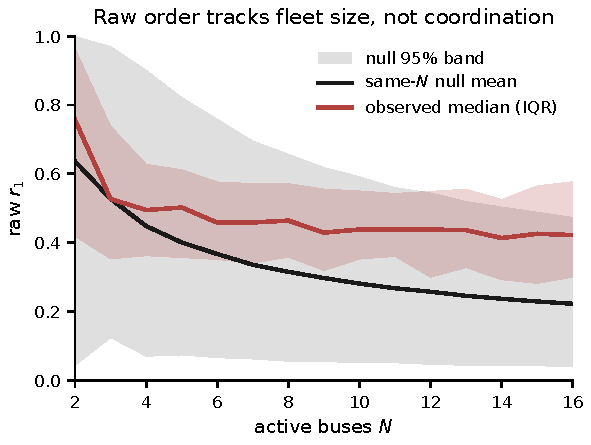
\includegraphics[width=\columnwidth]{01_raw_r1_by_fleet_size.pdf}
\caption{Raw order has a moving finite-size baseline.  Observed medians should be compared with
the same-$N$ null, not across fleet sizes directly.  The grey region is the null 95\% interval;
the red region is the observed interquartile range.}
\label{fig:finite}
\end{figure}

\begin{figure}[t]
\centering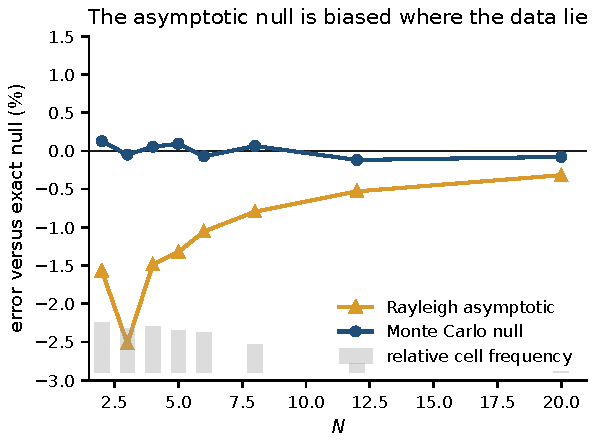
\includegraphics[width=\columnwidth]{02_null_approximation_error.pdf}
\caption{The Rayleigh approximation is biased where most cells lie, whereas the simulated null
agrees with the exact Kluyver mean within Monte Carlo error.  Bars show the relative frequency of
the displayed $N$ values, not an additional response variable.}
\label{fig:null}
\end{figure}

\section{Model discrimination}

The mean-field Kuramoto model assumes constant natural phase velocity, attractive all-to-all
coupling, a closed ring, a fixed frequency distribution, and a large ensemble.  A bus route has
local directed interaction, terminal resets, changing membership, and median $N=6$.  Computing a
Kuramoto order parameter therefore does not establish Kuramoto dynamics.

For the nearest-neighbour Newell--Potts mechanism, if dwell increment is $kh_{n,j}$, headway
perturbations evolve as
\begin{equation}
h_{n,j+1}=(1+k)h_{n,j}-kh_{n-1,j}.
\end{equation}
Substituting $h_{n,j}=A^j e^{i\theta n}$ yields
\begin{align}
A(\theta)&=(1+k)-ke^{-i\theta},\\
|A|^2&=(1+k)^2-2k(1+k)\cos\theta+k^2.
\end{align}
Thus $|A(0)|=1$, while $|A(\theta)|>1$ for every $k>0$ and nonzero $\theta$.  The idealized
model has no positive load threshold: instability accelerates continuously with $k$.  This is a
theoretical comparator, not proof that observed cells obey the model.

\begin{figure}[t]
\centering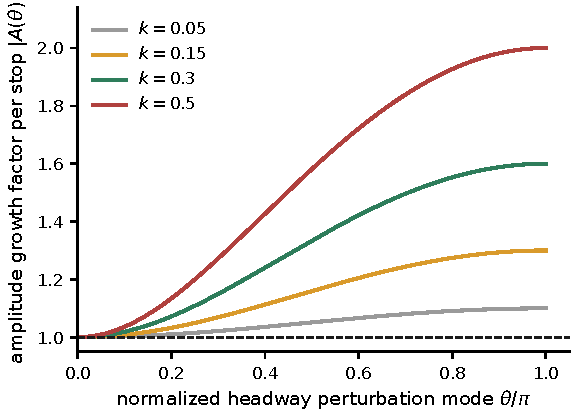
\includegraphics[width=\columnwidth]{08_newell_potts_theory_curves.pdf}
\caption{Newell--Potts growth factors.  The uniform-shift mode $\theta=0$ is neutral; every
nonzero mode grows for every positive $k$.  Hence the idealized bus-following theory predicts no
positive load threshold.}
\label{fig:newelltheory}
\end{figure}

\section{Results}

\subsection{Raw and corrected weekend comparisons}

In raw arc phase, weekend minus weekday $r_1$ is $+0.045$ (95\% CI $[0.036,0.055]$), while mean
fleet size falls from 7.99 to 4.47.  Matching exactly within $N$ reduces the raw contrast to
$+0.014$.  Under the arc-uniform correction the marginal contrast reverses,
$\Delta\rexc=-0.068$ $([-0.087,-0.049])$, whereas the exact-$N$-matched contrast is
$+0.012$ $([-0.009,+0.031])$.

Across all seven specifications, 30 of 35 marginal corrected contrasts are negative and all 35
matched point estimates are positive; 24 matched confidence intervals exclude zero.  This is not
a contradiction.  The marginal estimand includes the weekend supply pathway through $N$; the
matched estimand asks for a day-type association at the same active fleet size.  Neither is a
causal weekend treatment effect.

\begin{figure}[t]
\centering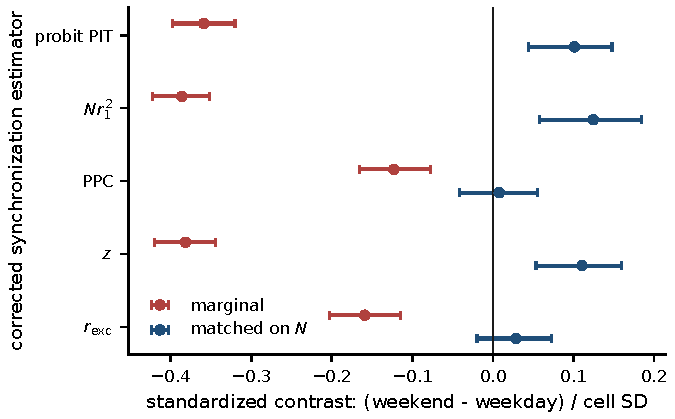
\includegraphics[width=\columnwidth]{03_weekend_contrasts.pdf}
\caption{Marginal and exact-$N$-matched weekend contrasts, scaled by each estimator's empirical
standard deviation.  All estimators change direction with the estimand.  The comparison is about
conditioning on fleet size, not choosing the estimator that gives a preferred sign.}
\label{fig:weekend}
\end{figure}

\begin{table}[t]
\centering
\caption{Weekend--weekday contrasts, arc phase and uniform null.}
\begin{tabular}{lrr}
\toprule
Estimator & Marginal & Matched on $N$\\
\midrule
Raw $r_1$ & $+0.045$ & $+0.014$\\
$\rexc$ & $-0.068$ & $+0.012$\\
$z$ & $-0.458$ & $+0.133$\\
PPC & $-0.043$ & $+0.003$\\
$Z_R$ & $-0.580$ & $+0.187$\\
probit PIT & $-0.399$ & $+0.112$\\
\bottomrule
\end{tabular}
\label{tab:weekend}
\end{table}

\subsection{Load response: crossover without demonstrated criticality}

A random-intercept model with line-direction effects, standardized $N$, time-of-day harmonics,
weekend, rain, and a load--rain interaction gives a standardized load coefficient of 0.04256
($p<10^{-15}$).  This is an association with realized load.  On the same fixed-effect frame, a
piecewise curve has AIC 10308.21, compared with 10334.61 for linear and 10396.36 for sigmoid.  Its
descriptive scale is $\lambda_c=135.74$ boardings per active bus.

\begin{figure}[t]
\centering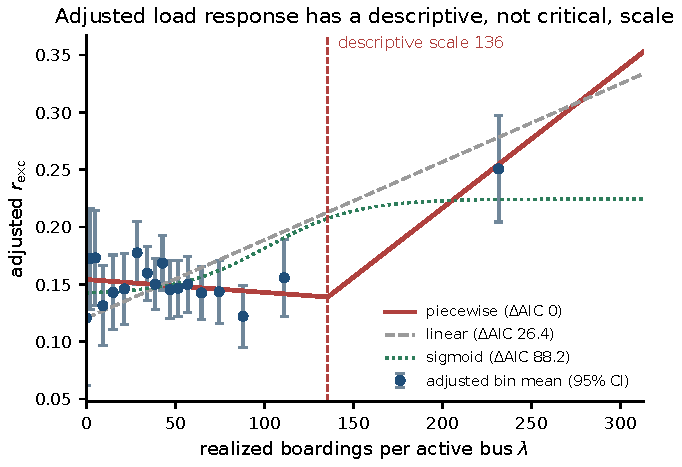
\includegraphics[width=\columnwidth]{18_corrected_load_response_models.pdf}
\caption{Adjusted corrected order versus realized load.  Points are equal-count-bin means of the
piecewise-model partial residual with 95\% normal intervals; curves hold line-direction and
non-load controls at their sample-average values.  AIC favors a descriptive change in slope near
136, but a breakpoint is not a critical point.}
\label{fig:load}
\end{figure}

We predeclare three signatures of criticality: an interior susceptibility peak, bimodality or
coexistence near the candidate scale, and stability of the apparent scale across $N$.  The first
two fail and only $N$-stability passes ($|\mathrm{corr}(\lambda_{peak},N)|=0.282$).  The verdict is
one of three signatures, consistent with a smooth crossover and no demonstrated criticality.

A free-exponent collapse $r=N^{-b}F((\lambda-\lambda_c)N^a)$ is non-diagnostic.  In the new raw
rebuild, the whole-route narrow-start solution improves the objective by 3.43 (permutation
$p=0.167$), while a broad start gives 10.01 at a different exponent-boundary solution.  The
interior fit is likewise start-sensitive and boundary-limited.  We therefore set
\texttt{collapse\_identified=false} and interpret neither exponents nor permutation values as
transition evidence.

\begin{table}[t]
\centering
\caption{Criticality decision gate.}
\small
\begin{tabularx}{\columnwidth}{@{}Xlc@{}}
\toprule
Signature & Result & Pass\\
\midrule
Interior susceptibility peak & absent & no\\
Near-scale bimodality & weaker than off-scale & no\\
Scale stable across $N$ & $|r|=0.282$ & yes\\
Free-exponent collapse & not identified & not scored\\
\bottomrule
\end{tabularx}
\label{tab:critical}
\end{table}

The corrected Daido harmonics are nearly flat: arc-phase means are 0.157, 0.159, and 0.149 for
$m=1,2,3$; time-phase means are 0.271, 0.293, and 0.275.  A broad single von Mises cluster tuned at
$m=1$ decays toward zero at higher harmonics.  Flat harmonics therefore describe compact clumps,
not the emergence of one smooth mean-field phase density.

\subsection{Route position is a first-class variable}

Even after layover exclusion, 27.19\% of active bus-hours lie within 2\% of a route end and an
additional 24.18\% lie between 2\% and 10\%; only 48.63\% are in the 10--90\% interior.  Median
matching residuals are similar in the three zones (4.24, 3.87, and 4.14 m), so the boundary mass
is not a projection artifact.

\begin{figure}[t]
\centering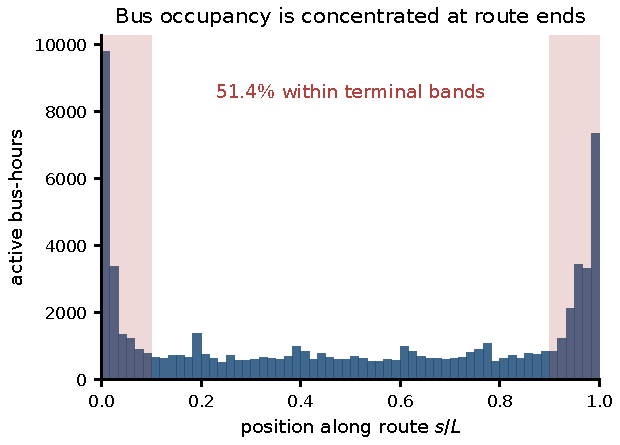
\includegraphics[width=\columnwidth]{04_bus_position_distribution.pdf}
\caption{Distribution of representative bus-hour positions.  The shaded outer deciles contain
51.37\% of active bus-hours after the layover rule.  The plot establishes occupancy, not the cause
of terminal waiting.}
\label{fig:position}
\end{figure}

Order parameters are recomputed inside each zone, with a new within-zone $N$.  Terminal cells have
mean $\rexc=0.9974$, near-terminal cells 0.9186, and interior cells $-0.1887$.  Negative interior
excess means more even spacing than the specified same-$N$ uniform null; it is consistent with a
splay-like state but does not by itself prove successful dispatch control.

\begin{figure}[t]
\centering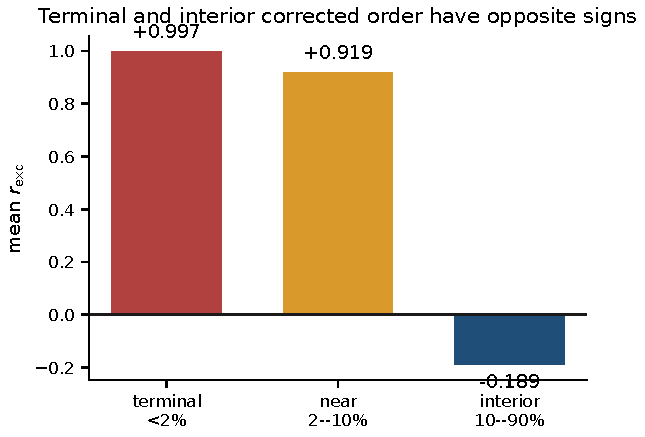
\includegraphics[width=\columnwidth]{05_synchronization_by_zone.pdf}
\caption{Corrected order changes sign by route zone.  Terminal concentration is nearly perfect by
geometry, while interior vehicles are more evenly spaced than the reference null.  These are
zone-specific estimands because $N$ is recomputed within each zone.}
\label{fig:zones}
\end{figure}

The standardized whole-route load coefficient in a line-direction fixed-effect model is 0.03758
(95\% CI $[0.01097,0.06420]$, $p=0.00565$).  No zone has a detectable within-zone load coefficient:
the interior estimate is 0.00111 ($[-0.02460,0.02683]$, $p=0.9325$).  Directly adding terminal
fraction to the whole-route model reduces the load coefficient to 0.02106, a 44\% attenuation;
terminal fraction itself has coefficient 1.2386 ($p\approx8.2\times10^{-182}$).  Thus the
whole-route association is substantially compositional, not proven to be purely compositional.

\begin{figure}[t]
\centering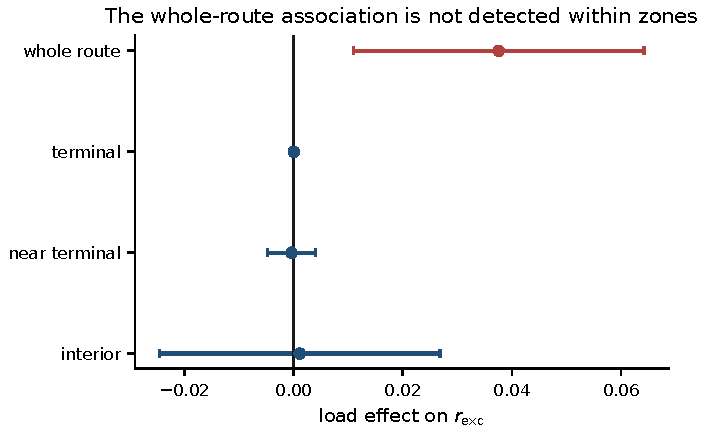
\includegraphics[width=\columnwidth]{07_load_effect_by_zone.pdf}
\caption{Standardized load coefficients with line-direction fixed effects, $\log N$ control, and
clustered 95\% intervals.  The association is detected for the whole-route mixture but not within
terminal, near-terminal, or interior zones.  Absence of detection is not proof of exact zero.}
\label{fig:zoneload}
\end{figure}

Trimming 2\% from both ends changes arc-phase mean $\rexc$ from 0.155 to $-0.120$; at 5\% it is
$-0.223$.  More severe trimming eventually removes genuine route and reduces median $N$ to three,
so 2--10\% is the informative range.  Each trim is a different estimand because both the phase
distribution and fleet size change.

\begin{table}[t]
\centering
\caption{Corrected order and load association by route zone.}
\begin{tabular}{lrrr}
\toprule
Zone & Cells & mean $\rexc$ & load coef.\\
\midrule
Terminal $<2\%$ & 5,044 & 0.9974 & 0.00004\\
Near 2--10\% & 3,980 & 0.9186 & $-0.00038$\\
Interior 10--90\% & 7,738 & $-0.1887$ & 0.00111\\
Whole route & 10,135 & 0.1574 & 0.03758\\
\bottomrule
\end{tabular}
\label{tab:zones}
\end{table}

\subsection{Mechanisms: amplification and common shocks}

Headway CV rises downstream across the 10--90\% interior: the mean slope is 0.1281
($p=1.32\times10^{-68}$).  In 5,049 cells with complete driver data, inherited initial CV is the
dominant standardized predictor of remaining growth ($-0.2917$); the negative sign is a ceiling
effect because already-irregular cells have less room to worsen.  Realized load is much smaller
(0.0149, CI $[0.0018,0.0280]$); route length, stop density, and sinuosity are unresolved.

The empirical Newell parameter $k=$ mean dwell per stop divided by mean headway has median 0.0477.
Across 5,900 cells, median measured growth is 0.0139 per stop, compared with fastest-mode prediction
0.0911 and mode-1 prediction 0.0162.  Seventy-one percent of cells grow, but predicted and measured
growth correlate only 0.0198 ($p=0.1277$).  The idealized theory gives a plausible scale and
no-threshold mechanism but does not rank which cells amplify.

\begin{figure}[t]
\centering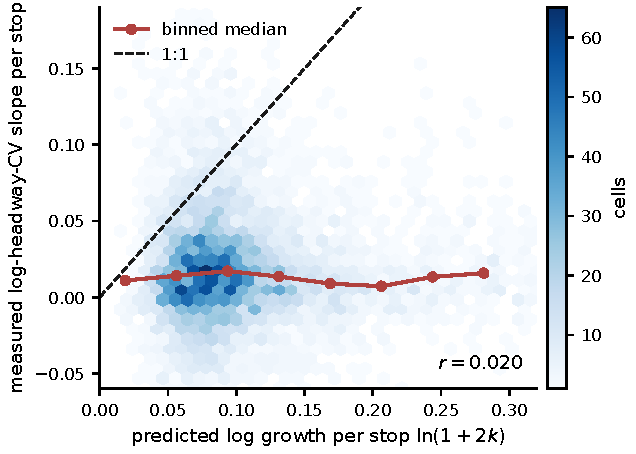
\includegraphics[width=\columnwidth]{09_newell_potts_empirical_test.pdf}
\caption{Measured versus Newell--Potts fastest-mode growth.  Binned medians remain nearly flat and
the cell-level correlation is 0.020.  Agreement of an average order of magnitude must not be
mistaken for predictive validation.}
\label{fig:newellemp}
\end{figure}

The GPS-derived dwell mediation indirect effect is $5.49\times10^{-5}$ with bootstrap CI
$[-0.000206,0.000401]$.  This is inconclusive, not evidence against passenger dwell: tickets are
not linked to individual vehicles and GPS dwell is noisy.

For overlapping route pairs, shared-trunk minus off-trunk correlation is 0.05325 (95\% CI
$[0.02444,0.08207]$).  After both line series are residualized on shared-segment mean speed, the
gap falls to 0.01273 ($[-0.01808,0.04889]$), retaining 24\%.  Only 5.88\% of pairs have significant
nonzero-lag peaks, and transfer-entropy directional asymmetry is null ($p=0.652$).  The evidence is
largely consistent with common road-state exposure; speed control could also absorb part of a
genuine coupling channel.

\begin{figure}[t]
\centering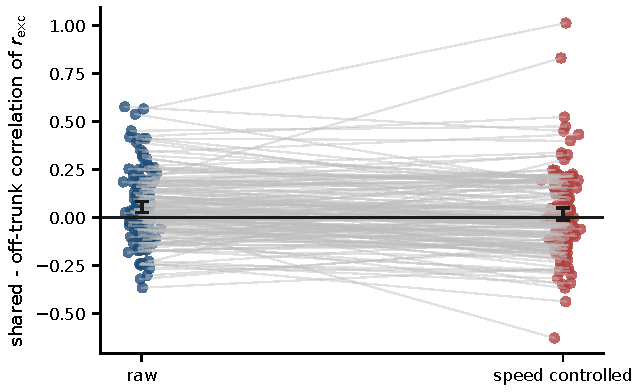
\includegraphics[width=\columnwidth]{15_corridor_speed_control_effect.pdf}
\caption{Within-pair shared-minus-off-trunk correlations before and after controlling shared
speed.  Grey lines preserve pair identity; black intervals summarize the pair distribution.  The
controlled mean spans zero, supporting a largely common-shock interpretation.}
\label{fig:corridor}
\end{figure}

\begin{figure}[t]
\centering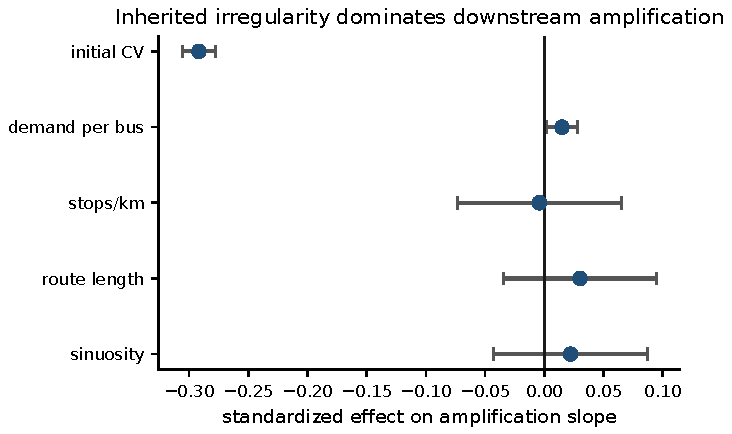
\includegraphics[width=\columnwidth]{17_amplification_driver_coefficients.pdf}
\caption{Standardized predictors of downstream amplification with 95\% intervals.  The large
negative initial-CV coefficient represents limited remaining growth, not a stabilizing effect of
irregularity.}
\label{fig:drivers}
\end{figure}

\section{Discussion}

The main result is a measurement result with physical consequences.  Raw $r_1$ is high in small
fleets even without coordination, so conditions that change $N$ inherit a false coherence contrast.
Same-$N$ correction is necessary, but it is not sufficient: the corrected statistic still depends
on the phase coordinate, the occupancy null, and where buses sit on an open route.  PPC reduces
finite-sample bias under alternatives, while explicit null and phase sensitivity reveal which
assumptions drive interpretation.

The data support a smooth operational crossover, not a demonstrated critical transition.  AIC
preference for a piecewise curve identifies a useful descriptive scale, but susceptibility and
coexistence fail, and free-exponent scaling is not identified.  This result is physically coherent:
the appropriate nearest-neighbour theory is unstable for every positive $k$, whereas mean-field
Kuramoto assumptions are violated by directed coupling, terminal resets, varying $N$, and frequency
heterogeneity.

Spatial mixture is the strongest empirical explanation for apparent whole-route synchronization.
The result is not merely that terminals contain many buses; it is that terminal and interior order
have opposite signs, zone-specific load effects are absent, and direct terminal-fraction control
substantially attenuates the whole-route coefficient.  The residual coefficient and changed
within-zone $N$ prevent a claim of complete mediation.

Operationally, inherited irregularity and shared road conditions are more informative than a
single passenger-load threshold.  Interventions aimed at headway regularization and common corridor
conditions are more directly supported than policies based on an inferred critical coupling.

\section{Limitations}

The missing vehicle crosswalk confines load to route-hour resolution and makes vehicle-level dwell
mediation unidentifiable.  Realized load divides by endogenous supply.  Representative midpoint
positions compress within-hour trajectories, while zone restriction and trimming change both
occupancy and $N$.  Nulls assume conditional exchangeability even though physical interactions are
directed.  Speed residualization may remove both common shocks and part of genuine coupling.  The
scaling objective has three free parameters, five strata, discontinuous bin membership, and boundary
solutions.  Finally, the record covers 19 days in one city; replication should test whether the
large terminal mass is specific to this network.

\section{Conclusion}

The Niter\'oi data can be made to look Kuramoto-like with a conventional order parameter, but that
appearance does not identify critical synchronization.  Exact finite-size reasoning changes the
baseline; marginal and fleet-size-conditional weekend comparisons answer different questions;
route-position analysis reveals a terminal/interior mixture; and common-speed control removes most
shared-corridor coherence.  The surviving physical picture is an unconditional, smoothly
load-modulated operational instability embedded in boundary occupancy and common road shocks, not
a demonstrated city-scale critical transition.

\section*{Reproducibility statement}

All numbers, tables, and independent figures in this report were regenerated from the released raw
data in one corrected execution on 21 August 2026.  The run uses continuous route geometry, explicit
input/output paths, fixed random seeds for inferential simulations, 26 passing unit tests, seven
phase--null specifications, and an explicit non-identification gate for scaling collapse.

\begin{thebibliography}{14}\small
\bibitem{newell64} G. F. Newell and R. B. Potts, ``Maintaining a bus schedule,'' Proc. 2nd Australian Road Research Board Conference (1964), 388--393.
\bibitem{saw19} V.-L. Saw et al., ``Bus bunching as a synchronisation phenomenon,'' Scientific Reports 9, 6887 (2019).
\bibitem{strogatz00} S. H. Strogatz, ``From Kuramoto to Crawford,'' Physica D 143, 1--20 (2000).
\bibitem{kuramoto75} Y. Kuramoto, International Symposium on Mathematical Problems in Theoretical Physics, Lecture Notes in Physics 39 (1975), 420.
\bibitem{kluyver05} J. C. Kluyver, ``A local probability problem,'' Proc. Sect. Sci. Koninklijke Akademie van Wetenschappen 8, 341--350 (1905).
\bibitem{vinck10} M. Vinck et al., ``The pairwise phase consistency,'' NeuroImage 51, 112--122 (2010).
\bibitem{daido90} H. Daido, ``Intrinsic fluctuations and a phase transition,'' Journal of Statistical Physics 60, 753--800 (1990).
\bibitem{chew19} L. Y. Chew, V.-L. Saw, and Y. E. I. Pang, ``Stability of anti-bunched buses and local unidirectional Kuramoto oscillators,'' arXiv:1912.06470 (2019).
\bibitem{daganzo09} C. F. Daganzo, ``A headway-based approach to eliminate bus bunching,'' Transportation Research B 43, 913--921 (2009).
\bibitem{gershenson09} C. Gershenson and L. A. Pineda, ``Why does public transport not arrive on time?'' PLoS ONE 4, e7292 (2009).
\bibitem{hong07} H. Hong et al., ``Entrainment transition in populations of random frequency oscillators,'' Physical Review Letters 99, 184101 (2007).
\end{thebibliography}
\end{document}
